% !Mode:: "TeX:UTF-8" 
\section{国内外在该方向的研究现状及分析}
\subsection{国外研究现状}

“不确定性”和“风险”是各个学术领域均比较关注的一个研究问题。本节简要归纳不确定性的分类、度量和各类不同的处理对策,思路如图~\ref{uc_ways}~所示。

\begin{figure}[htbp]
\centering
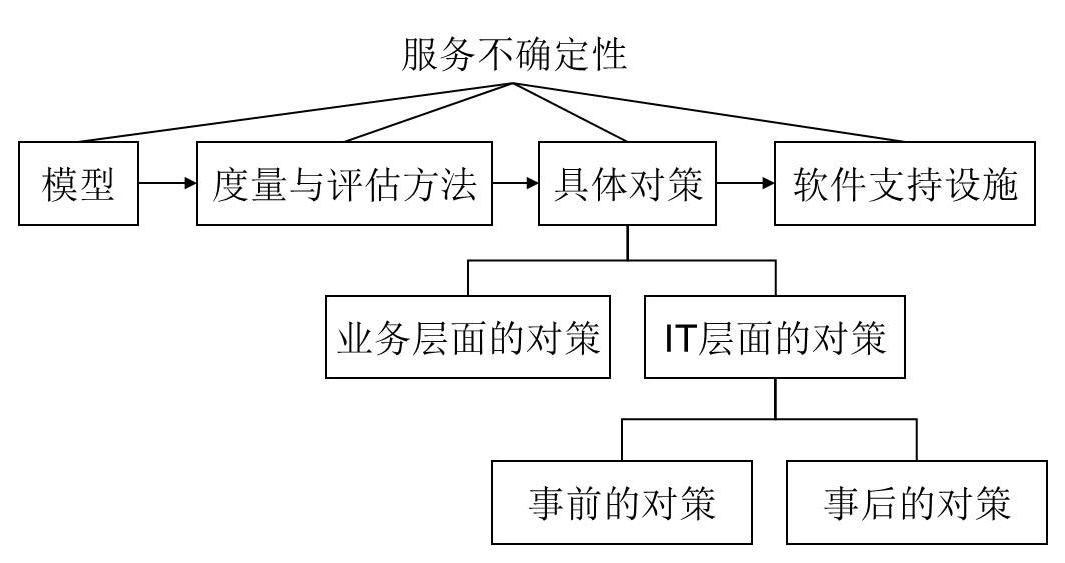
\includegraphics[width = 0.4\textwidth]{uc_ways}
\caption{按需应变的服务不确定性自适应决策}\label{uc_ways}
\vspace{-1em}
\end{figure}

在按需服务环境中,服务执行之前供需双方在性能、可靠性和可用性等~QoS~方面达成服务级别协议~(SLA)~。目前得以广泛应用的~Web Service Level Agreement (WSLA)~是一种用于定义和监测~web~服务的~SLA~描述语言和框架\citeup{keller2003wsla},为~SLA~的建模、扩展、度量和监控提供支持。文献\cite{kokash2007evaluating}\cite{chan2009fault}\cite{ardagna2006faults}对服务运行时可能发生的不确定性进行了不同角度的分类,从不确定性发生的层次(应用层面、服务层面、基础设施/中间件层面)、不确定性发生时的表现(服务/数据缺失、非期望的服务行为、性能问题、协议违反)等方面阐述了不确定性的含义,通过基于SLA的风险度量与估算方法协助发现不确定性及其影响\citeup{michalk2010risk}。

服务不确定性与其可靠性息息相关,因此可采用可靠性保障的方法来解决~web~服务中的不确定性问题\citeup{subramanian2008enhancement},在最初构建服务方案时就考虑可能面临的风险,将可靠性、不确定性等因素加入到服务选择与服务组合模型/算法中,以降低未来执行中的风险。使用随机~Petri~网等工具对~web~服务组合方案进行建模并计算其可靠性\citeup{zhong2008reliability},或者将服务发生风险时的依赖关系作为服务组合的可靠性优化依据\citeup{liu2009risk},通过~Markov~决策过程(MDP)等方法来选择最符合客户风险偏好的可靠服务\citeup{harney2008selective}\citeup{gao2011reliability}。

为了在服务执行产生不确定事件时能够通过恢复机制来保障可靠性\citeup{chan2009design},可基于冗余策略预先配置备用服务或多个替代配置方案(配置树、执行计划)来提升服务方案的容错能力\citeup{kokash2006service},目标是使服务方案具备自我治愈的能力\citeup{ardagna2006faults}。当现有服务无法正常执行时直接由备选服务接替执行,也可采用备选流程的方式,在当前流程出现问题时直接切换到备选流程。为此需在服务建模阶段考虑各种不确定性,对建模元素的实现机制和应用场景进行扩展以提高模型描述能力和适应性\citeup{fan2002service}。

\subsection{国内研究现状}

服务执行过程中的典型动态自适应策略包括:服务替换、服务重组等服务重配置方法、恢复与补偿机制等策略\citeup{erradi2006recovery}。服务替换考虑服务的功能和非功能特性,基于服务的参数类型等静态属性和动态行为特性的匹配保证替换前后服务过程功能的一致性,基于客户的QoS偏好对服务效用进行度量来保证和优化替换后的服务质量\citeup{athanasopoulos2009service},并引入context对服务的可替换性进行判断\citeup{pathak2007context}。

服务重组分为服务的大规模重选取和服务路径的重规划。文献\cite{bouhini2010discovery}使用服务片段作为重规划的基本单元以提升效率,文献\cite{bucchiarone2010design}提出了一组系统化的原则和指南,指导设计者如何构造/重规划适应变化的服务。为降低重组代价,对服务过程内处于不同执行状态的部分进行划分,每次尝试都期望在尽量小范围内弥补不确定性产生的后果,并在尝试失败后逐渐扩大重组范围\citeup{zhai2009soa}。还可使用修补技术对当前服务组合方案进行改变和增强,使之适应各类故障\citeup{yan2010self}。还可根据服务执行反馈的状况,采用进行持续规划\citeup{kaldeli2011continual},以适应执行过程中出现的各类不确定情况。

\subsection{国内外文献综述的简析}
如上所述,目前关于服务不确定性的研究已经有了丰富的研究,但尚显不足。

(1)~大部分研究者站在软件服务的开发、运行和维护的角度上,探讨“当某服务执行出现异常”之前或之后如何应对。而本课题站在客户或者中介方的角度,他们作为服务的使用者,不可能也无需了解软件服务的内部执行细节,只是从外部观测到各类异常的发生,而无法得知造成异常的原因(例如服务器内部出错、网络出错等)。在这种情况下,通过各类不确定性的决策方法,提高第三方服务中介所构造的整体服务方案适应不确定性的能力,是本课题的研究重点,也是区别于传统研究的观点之一。

针对此类问题,归纳起来,目前的研究主要分为两类:
a)~建模阶段对服务模型进行抗风险能力的增强,一旦运行时发现问题即可按预案进行应对;
b)~运行阶段对相关服务进行替换、重组或修补,并确保操作前后服务功能和QoS的一致性。
尚有以下两点不足:
a)~关注替换、重组、修补等单一决策动作如何操作、如何实施,对哪种动作的效果最优的考虑显得不足;
b)~决策目标定位在服务功能的相容性和~QoS~的可保障性,较少从经济角度考虑不确定性带来的时间和成本方面的损失。本文尝试着从这两点入手展开研究,试图将服务层面的不确定性与业务层目标结合起来,寻求处理不确定性的最优决策动作。

(2)~目前的研究通常将~business~和~IT~层面的不确定性割裂开来,分别研究。例如,针对供应链中的需求/供给/制造的不确定性,研究业务层面如何应对;针对底层的~web service~和服务系统执行中的出错、延迟、失败等不确定性,研究软件层面如何应对。但是二者本质上是有联系的,将它们关联起来并建立映射,是本课题的另一个观点。

针对此类问题,目前的研究主要是针对不同的业务情况采取不同的方法,其不足体现在两个方面,a)~没有对业务的不确定性进行系统化的分类处理,以至于不确定性的处理方案没有重用性和对处理结果统一的价值度量;b)~完全停留在~business~层面纯手工进行决策,忽略了~IT~手段可以辅助业务不确定性的决策,效率低下并且无法准确量化不确定性的决策的代价;

